\appendix
\chapter{Simple lattice Model}

\section{Propagation Algorithm}
\label{a:propagation}
Starting from simplicity, the model assumes local transmission between nearest neighbours. Local structure within the network is described by the von Neumann neighbourhood. To demonstrate the algorithm, take a $3 \times 3$  matrix $\mathbb{S}$ representing a small patch of forest, $1's$ represent trees in state $S$ while $0's$ represent insusceptible states $\emptyset$. An and infection matrix $\mathbb{I}$ is defined with an infected matrix element $I_{2,2}=2$. A removed matrix is also given by $\mathbb{R}$. At time $t=0$:
\begin{equation}
\mathbb{S}= \left( \begin{array}{ccc}
0 & 1 & 0\\
1 & 0 & 0\\
0& 1 & 0 \\
\end{array} \right)\qquad
\mathbb{I}= \left( \begin{array}{ccc}
0 & 0 & 0\\
0 &2 & 0\\
0& 0 & 0 \\
\end{array} \right)\qquad
\mathbb{R} = \left( \begin{array}{ccc}
0 & 0 & 0\\
0 & 0 & 0\\
0 & 0 & 0 \\
\end{array} \right)\qquad
\end{equation}

A centrally infected state in $\mathbb{I}$ can be seen\textemdash when $\mathbb{I}_{i,j} = 2,\ \mathbb{S}_{i,j} = 0$. The algorithm singles out neighbours surrounding the infected tree and generates random numbers $\{ R_{0,1},R_{1,0},R_{3,2}\}$. From this a potential infection matrix $\mathbb{I}^{'}$ is formed:

\begin{equation}
    \mathbb{I}^{'} = \begin{pmatrix}
        0 & R_{0,1} & 0 \\
        R_{1,0} & 2 & 0 \\
        0 & R_{2,1} & 0 
     \end{pmatrix}
\end{equation}

Each random number is generated uniformly between $[0,1] $. If  $R_{i,j} \leqslant \beta$ the infection jumps to site $(i,j)$. For example, assume $R_{0,1}\leqslant \beta$ and $R_{1,0}, R_{2,1} \geq \beta $, then at time $t=1$ the matrices are updated:

\begin{equation}
    \mathbb{S} = \left( \begin{array}{ccc}
    0 & 0 & 0\\
    1 & 0 & 0\\
    0& 1 & 0 \\
    \end{array} \right)\qquad
    \mathbb{I}= \left( \begin{array}{ccc}
    0 & 2 & 0\\
    0 & 3 & 0\\
    0& 0 & 0 \\
    \end{array} \right)\qquad
    \mathbb{R}= \left( \begin{array}{ccc}
    0 & 0 & 0\\
    0 & 0 & 0\\
    0 & 0 & 0\\
    \end{array} \right)\qquad
\end{equation}
    
When $\mathbb{I}_{i,j}=T+1, \mathbb{R}_{i,j} = 1$. The algorithm is repeated over a set time-horizon (typically $t=3000$) and eventually one of the three boundary conditions is met and the simulation ends. In python this is implemented by matrix operations:

\begin{lstlisting}[style=pythoncode,
    caption = An alorithm written in python to compute matrix equations and simulate disease spread. Code can be found in: \textcolor{red}{cite github repo?}.,
    label = py:rand]

def run(S, I, R, beta, T=10, L=500):
    """
    Run algorithm
    :param S: array-like, susceptible matrix
    :param I: array-like, infected matrix
    :param R: array-like, removed matrix
    :param beta: float, transmission probability
    :param T: int, infectious life-time of a tree
    :param L: int, lattice dimension
    :return:
    """
    # - Begin - #
    for t in range(3000):
            # nn : nearest neighbours, 
            # - single out vertical and horizontal nn respectively
            nn = np.roll(I, 1, axis=0) + np.roll(I, -1, axis=0)
            nn = nn + np.roll(I, 1, axis=1) + np.roll(I, -1, axis=1)
            nn = (nn * S) > 0  # sigle out susceptible trees only
            # inf_dyn : infection dynamics (a probability)
            inf_dyn = np.array(np.random.uniform(size=[L, L]) < beta)
            # add 1 to exitsting ifectes 
            # combine neaibourhood to infection status
            I = I + (I > 0) + 2 * nn * inf_dyn. 
            S = S * np.where(I > 0, 0, 1) # take away infecteds from S
            R = R + np.where(I == T, 1, 0)  # transition I to R
            R = np.array(R_tree > 0).astype(int). # Hold R as binary
            I = I * np.where(R > 0, 0, 1) # Remove infected status 
            # continue...
\end{lstlisting}

\section{SLM metrics}
\label{a:slm_metrics}

\textcolor{red}{Fill me with center of infectious mass information? If not, remove my reference in chapter \ref{chapter:SLM}}

\chapter{SLM\textemdash a mean-filed theory}

\label{a:slm-mean-field-theory}

Do, equations...
\blindtext

\chapter{SLM heterogeneous data\textemdash alternative metrics}
\label{a:slm_heterogeneous}

\begin{figure}
    \centering
    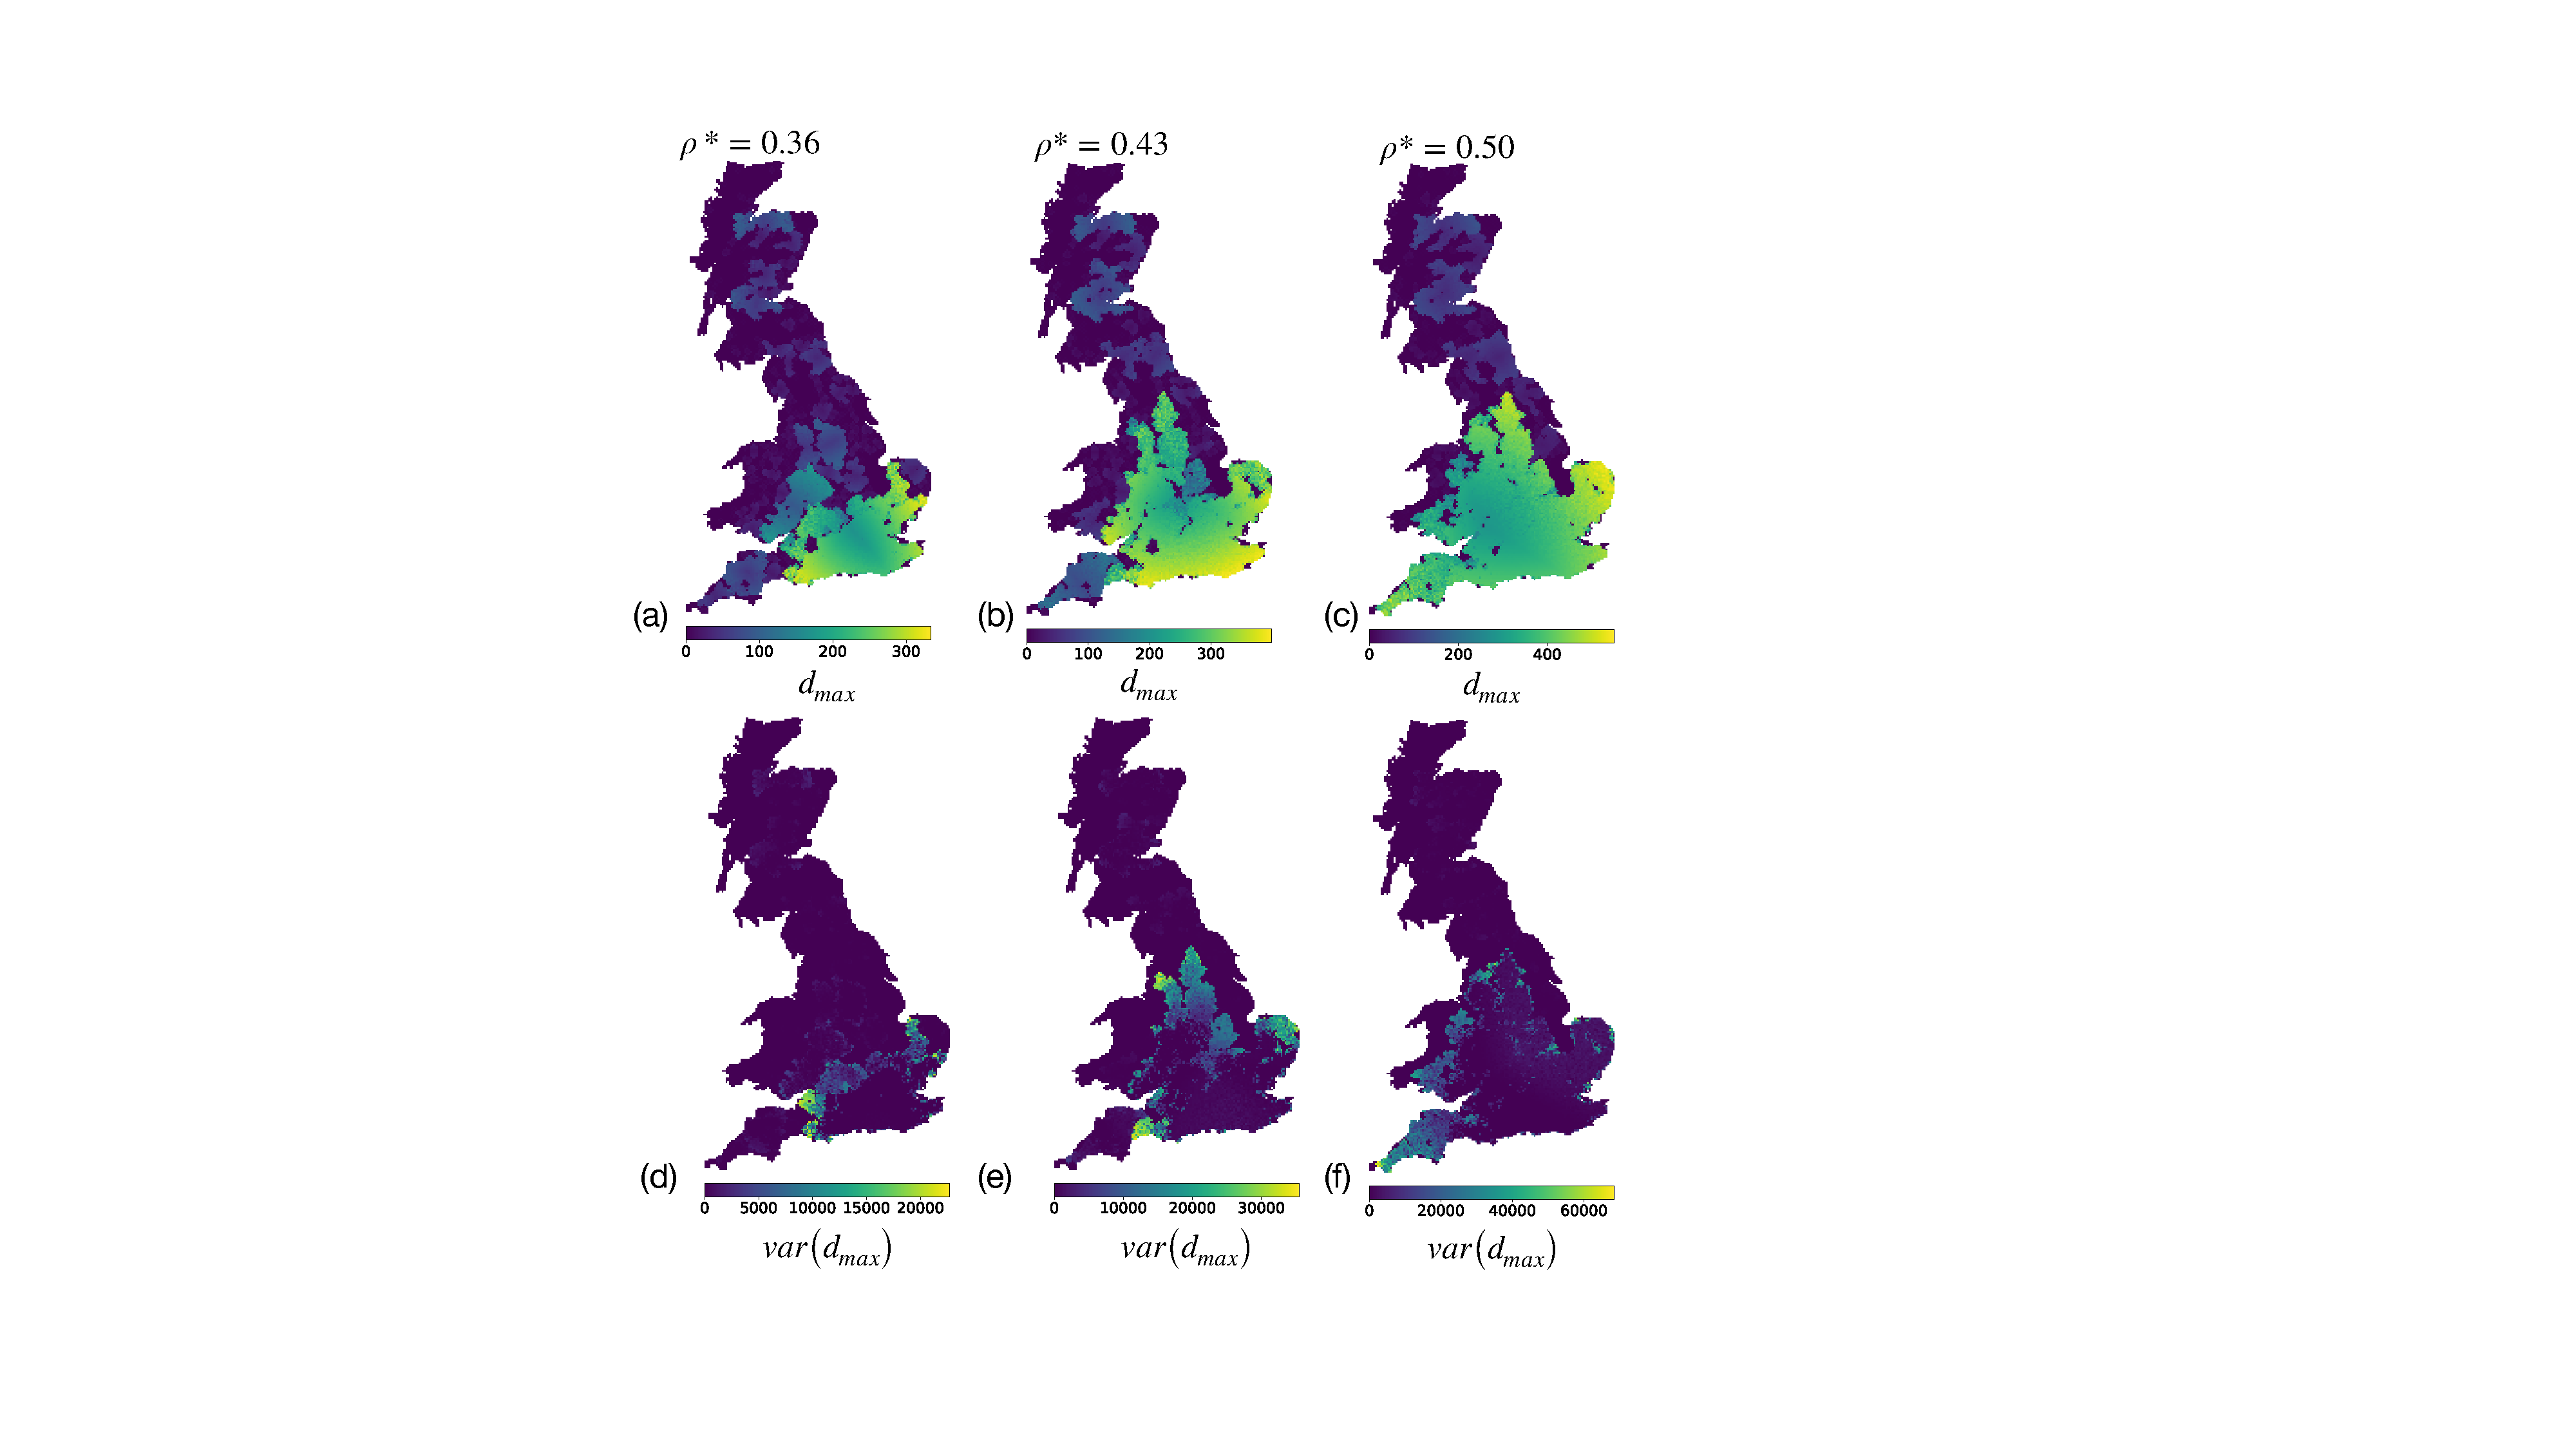
\includegraphics[scale=0.55]{appendix/figures/A-ch4figure1.pdf}
    \caption{The max-distance ($d_{max}$)} metric...
    \label{fig:my_label}
\end{figure}

\blindtext
\blindtext

\chapter{Non-local sub-grid model $R_0$ derivation}
\label{section:apendix_A}

Starting from an un-normalised Gaussian kernel $g(p, q; \ell) = \exp(\frac{p^2-q^2}{2\ell^2})$ and infectivity constant $\beta$, we may define the probability of position $q$ being infected due to an infected tree at $p$ as $Pr(q; p) = \beta g(p, q; \ell)$. The domain has tree density $\rho_0$ at time $t=0$ and trees transition through states: $S\rightarrow I\rightarrow R$, with $I$ lasting for $T$ time-steps. Considering the probability of point $q = (x, y)$ becoming infected on account of an infected tree located at the origin during the first time-step:
\begin{equation}
    Pr(x, y, t=0) = \beta \rho_0 \exp(-\frac{x^2+y^2}{2\ell^2})
\end{equation}{}
 Integrating this over an infinite domain gives $R_0(t=0)$ expected infections, given by:
\begin{equation}
    R_0(t = 0) = \beta \rho_0 \int^{\infty}_{-\infty} \exp(-\frac{x^2+y^2}{2\ell^2})dx dy= 2\pi\beta\rho_0\ell^2
\end{equation}{}
At time-step $t+1$ there are less trees to infect. Therefore tree density $\rho$ should also be considered as a monotonically decreasing function of time $\rho(t)$, and the number of expected infections should be given by:
\begin{equation}
    R_0(t) = 2\pi\beta\ell^2\rho(t)
    \label{eq:r0-A}
\end{equation}{}
 Considering density as a function of time\footnote{Density also varies with space as trees are removed quicker for regions closer around the primary infection. However, negating this lead to an easily solvable expression valid for lower-value regimes.} in a discrete domain of size $L$, the average decrease in tree density over one time-step is given by:

\begin{equation}
\label{eq:discrete-rho-t-A}
\begin{split}
\rho(t+1) & = \rho(t) - \frac{R_0(t)}{L^2} \\
 & = \rho(t)\Big(1 - 2\pi\beta\frac{\ell^2}{L^2} \Big)
\end{split}
\end{equation}

at $\rho(t=0)=\rho_0$, therefore, equation (\ref{eq:discrete-rho-t-A}) forms a series from which we may expand to give a continuous equation of $\rho$:
\begin{equation}
    \rho(t) = \rho_0 \big(1 - 2\pi\beta\frac{\ell^2}{L^2}\big)^t
\end{equation}{}
upon substitution back into equation (\ref{eq:r0-A}) we have an approximation for how the number of expected infections from one infected tree is expected to change over time:
\begin{equation}
    R_0(t) = 2\pi\beta\ell^2\rho_0 \big(1 - 2\pi\beta\frac{\ell^2}{L^2} \big)^t
    \label{eq:Rt-A}
\end{equation}{}
This expression is compared against numerical simulations in Fig \ref{fig:sgm-evol}(c). Then integrating over the infectious life-time $t=T$ gives an approximation to an effective reproductive number denoted by $R_0$:

\begin{equation} \label{eq1}
\begin{split}
R_0 & = 2\pi\beta\ell^2\rho_0 \int ^T _0 \big(1 - 2\pi\beta\frac{\ell^2}{L^2} \big)^t dt \\
 & = 2\pi\beta\ell^2\rho_0 \frac{ (1 - 2\pi \beta\frac{\ell^2}{L^2})^T - 1}{\ln(1 - 2\pi\beta\frac{\ell^2}{L^2})}
\end{split}
\end{equation}

(from $\int c^t dt = \frac{c^t}{\ln(c)}$). The expression for $R_0$ can be simplified by noting the pathogen is unlikely to infect trees beyond a distance of $3\ell$, therefore, we can replace the area of the domain with the area over three standard deviations (i.e. $9\pi\ell^2$), thus leading to the approximation:
\begin{align*}
    R_0 = 2\pi\beta\rho_0\ell^2 \frac{(1 - 2/9\beta)^T - 1}{\ln(1-2/9\beta)}
\end{align*}

\chapter{Percolation verses $R_0$}

\begin{figure}
    \centering
    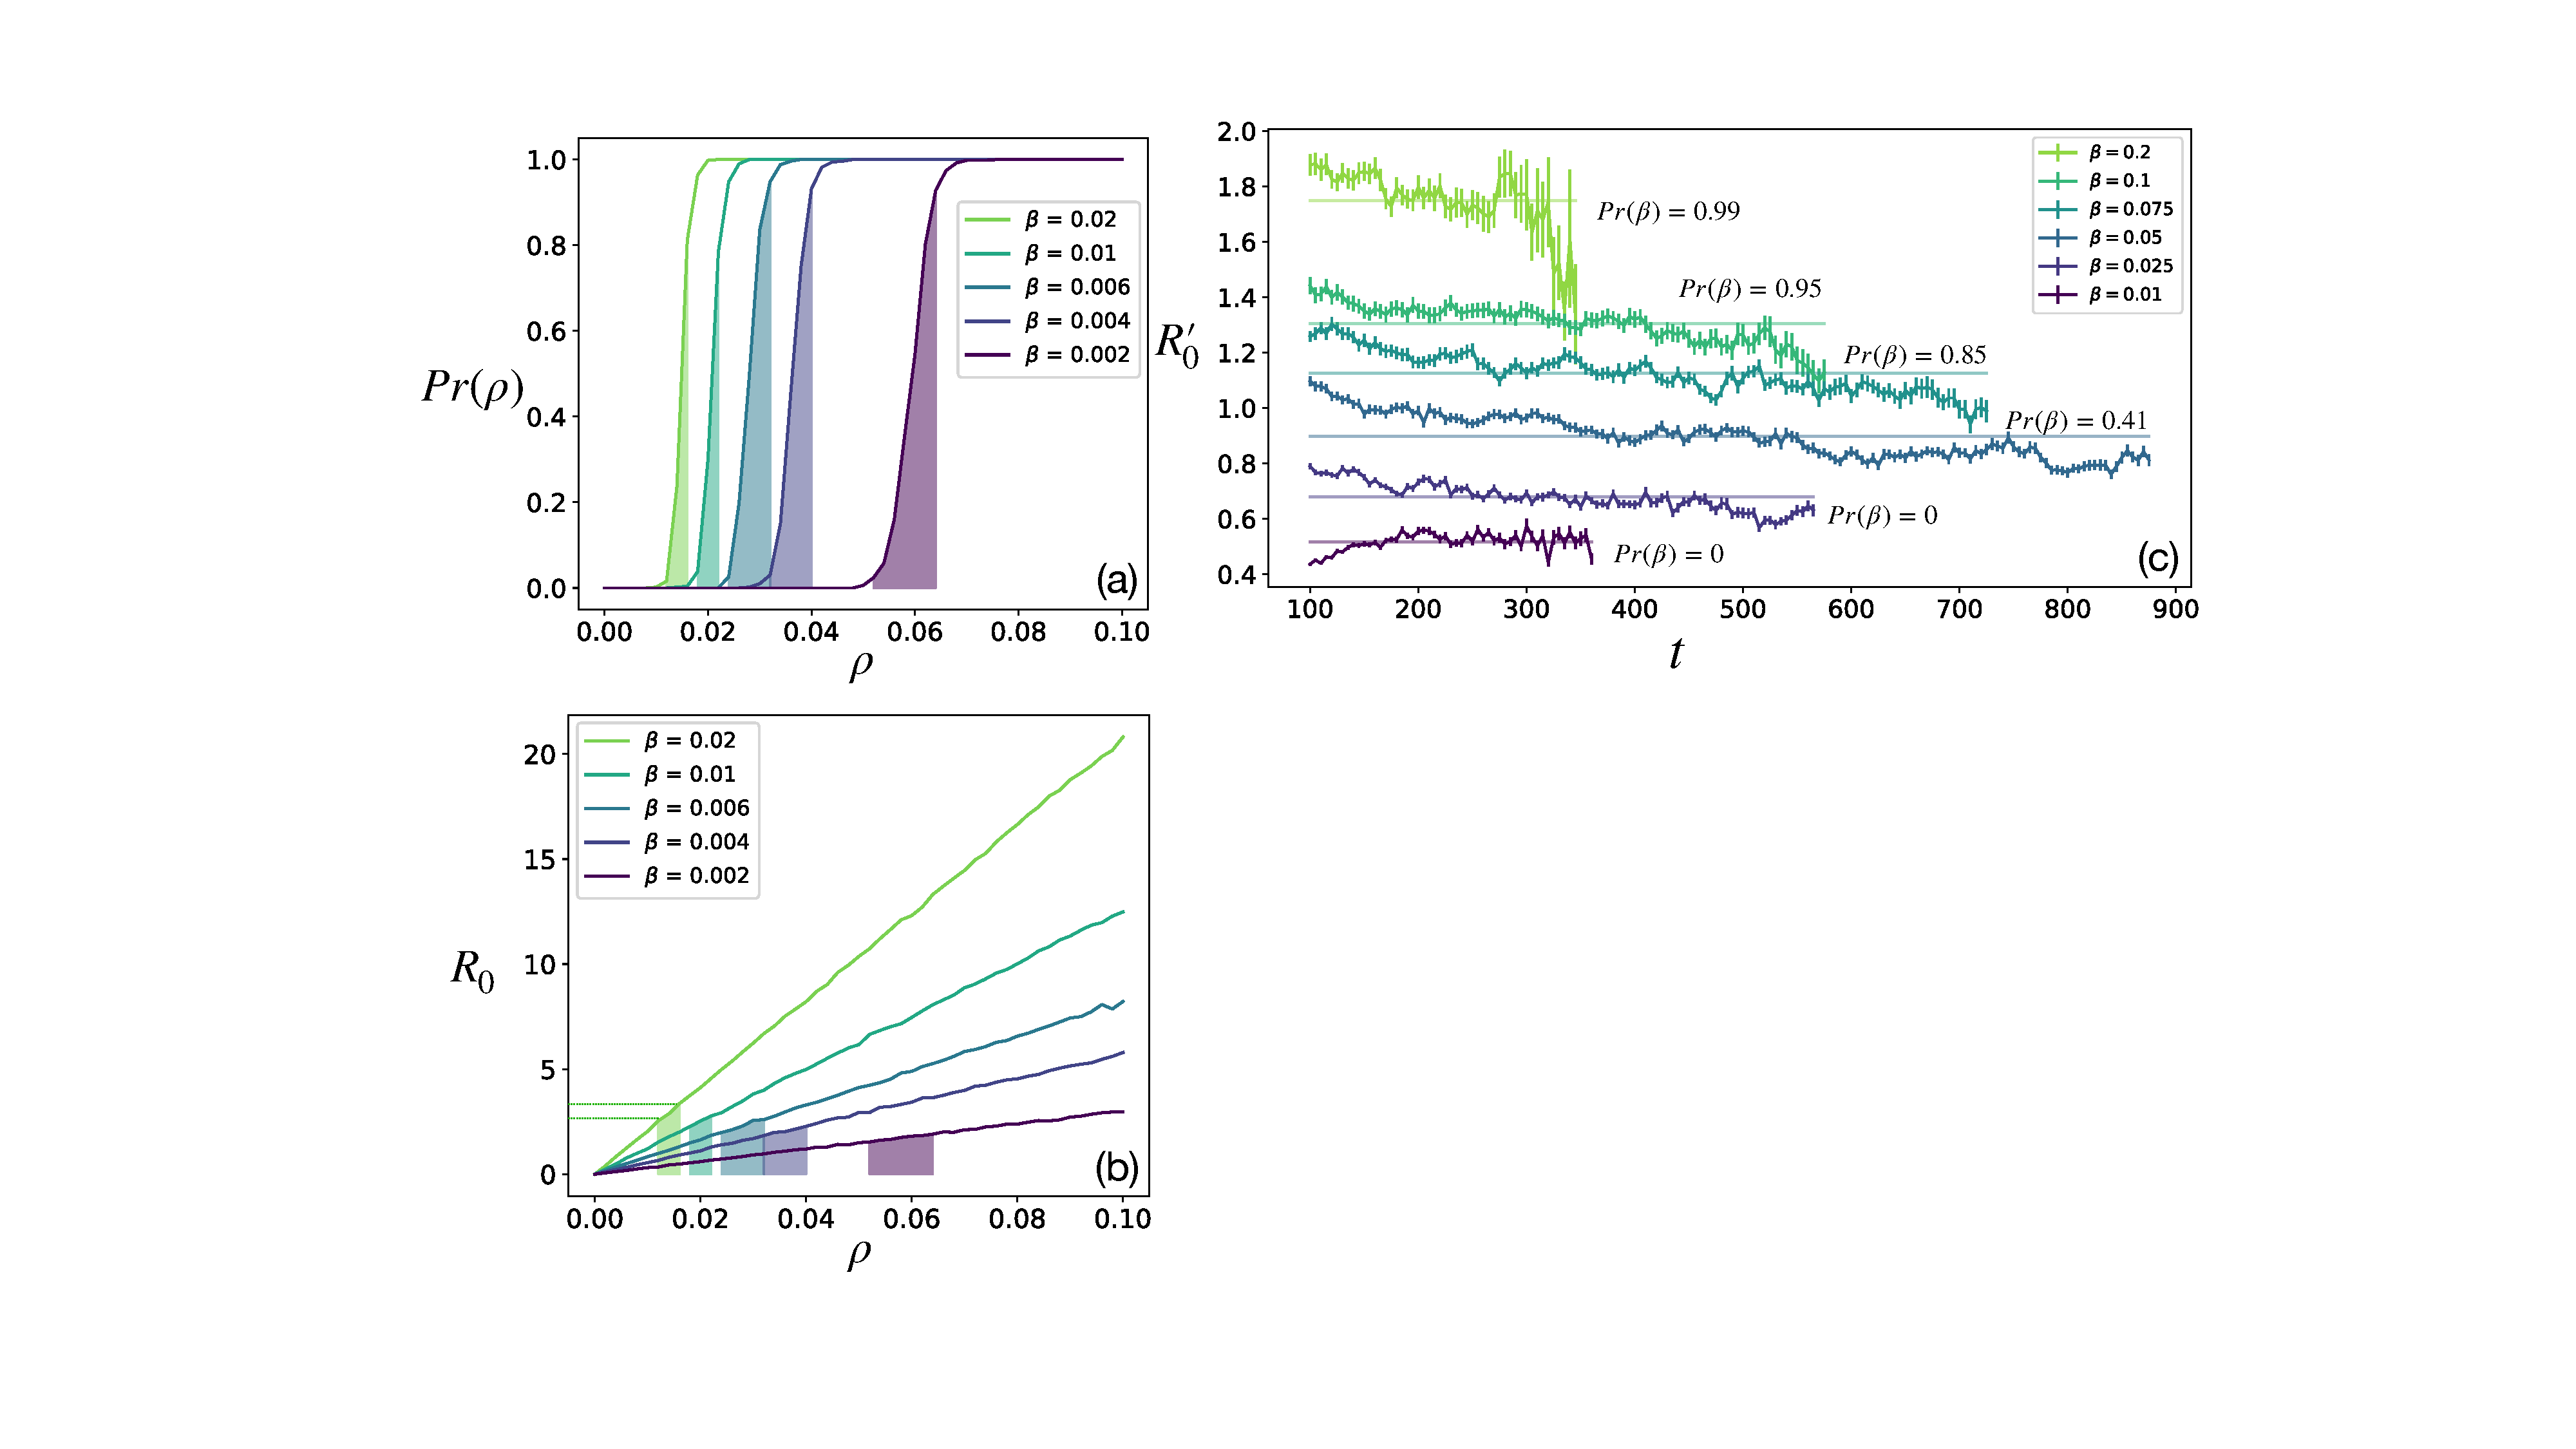
\includegraphics[scale=0.35]{appendix/figures/app1.pdf}
    \caption{Caption}
    \label{fig:my_label}
\end{figure}

\blindtext


\chapter{Regional containment: a formal explanation of the Cluster Fragmentation}
\label{section:alpha-step}
Given $\mathbf{C}$, a connected cluster in the $R_0$-map and threshold function $\phi(\alpha)$ defined by:
\begin{align}
\label{eq:alpha-step}
\phi(\alpha) = \left\{ \begin{array}{cc} 
                1 & R_0(i, j) \geq \alpha \\
                0 & R_0(i, j) < \alpha \\
                \end{array} \right.
\end{align}

where $(i,j)$ are spatial coordinates in $\mathbf{C}$ and $\alpha$ taking values in interval $[1, R_{max}]$. The value $R_{max}$ is the highest value of $R_0$ in $\mathbf{C}$. Applying the threshold function to $\mathbf{C}$ and moving in small discrete steps backward from $\alpha = R_{max}$ to $\alpha=1$ will create a set of binary maps from lower to higher pixel density. For example, applying the threshold function at $\alpha = R_{max}$ will map only the highest $R_0$ Ash tree patches in $\mathbf{C}$ to a value of one and produce a low density binary map. Whereas, at $\alpha=1$ all susceptible points will assume binary values of one and $\mathbf{C}$ will be defined exactly.\\

% Paragraph defining connected component analysis
Applying CCA over each binary map is performed through each $\alpha$-step in order to identify and label sub-clusters. At particular steps $\alpha \rightarrow \alpha - \delta\alpha$, $\mathbf{C}$ will begin to form when two\footnote{It is possible but unlikely that three or more sub-clusters suddenly connect to form $\mathbf{C}$ in the same step} distinct sub-clusters $\mathbf{C_1}$ and $\mathbf{C_2}$ suddenly connect when certain critical links become non-zero\textemdash analogous to the formation of a spanning cluster opening up in a percolation. When $\mathbf{C_1}$ and $\mathbf{C_2}$ abruptly merge and form the basis of $\mathbf{C}$, a large discontinuous jump in cluster size is detected. When a discontinuity is detected all spatial points $(i,j)$ which bridge the gap between $\mathbf{C_1}$ and $\mathbf{C_2}$ are found and felled.\\

Successive steps through $\alpha$ continue until $\alpha=1$ and critical links are felled for each discontinuity event. This prevents $\mathbf{C_1}$ and $\mathbf{C_2}$ from merging over $\alpha \in [1, R_{max}]$ and fragments the target-cluster $\mathbf{C}$ into two disconnected sub-clusters. The process is then repeated, the next cluster target will be either $\mathbf{C_1}$ or $\mathbf{C_2}$, whichever has the largest number of Ash trees. Iterating this $N$ times will yield $N+1$ disconnected cluster fragments.\\

\chapter{PDE modelling - finite difference solver}

\label{a:pde}

\begin{itemize}
    \item \textcolor{red}{How does the diffusion and growth parameters change the measured speed with dx and dt ? perhaps worth detailing...}
\end{itemize}
\blindtext

\blindtext


\chapter{Seasonal $SEIR$ model of Ash dieback}

\label{section:ga-SEIR-variant}
\begin{itemize}
    \item The Gaussian and inverse power-law models are distinct and could be considered to have different infecitivity parameters $\beta_{ga}$ and $\beta_{pl}$k.
\end{itemize}
\begin{figure}
    \centering
    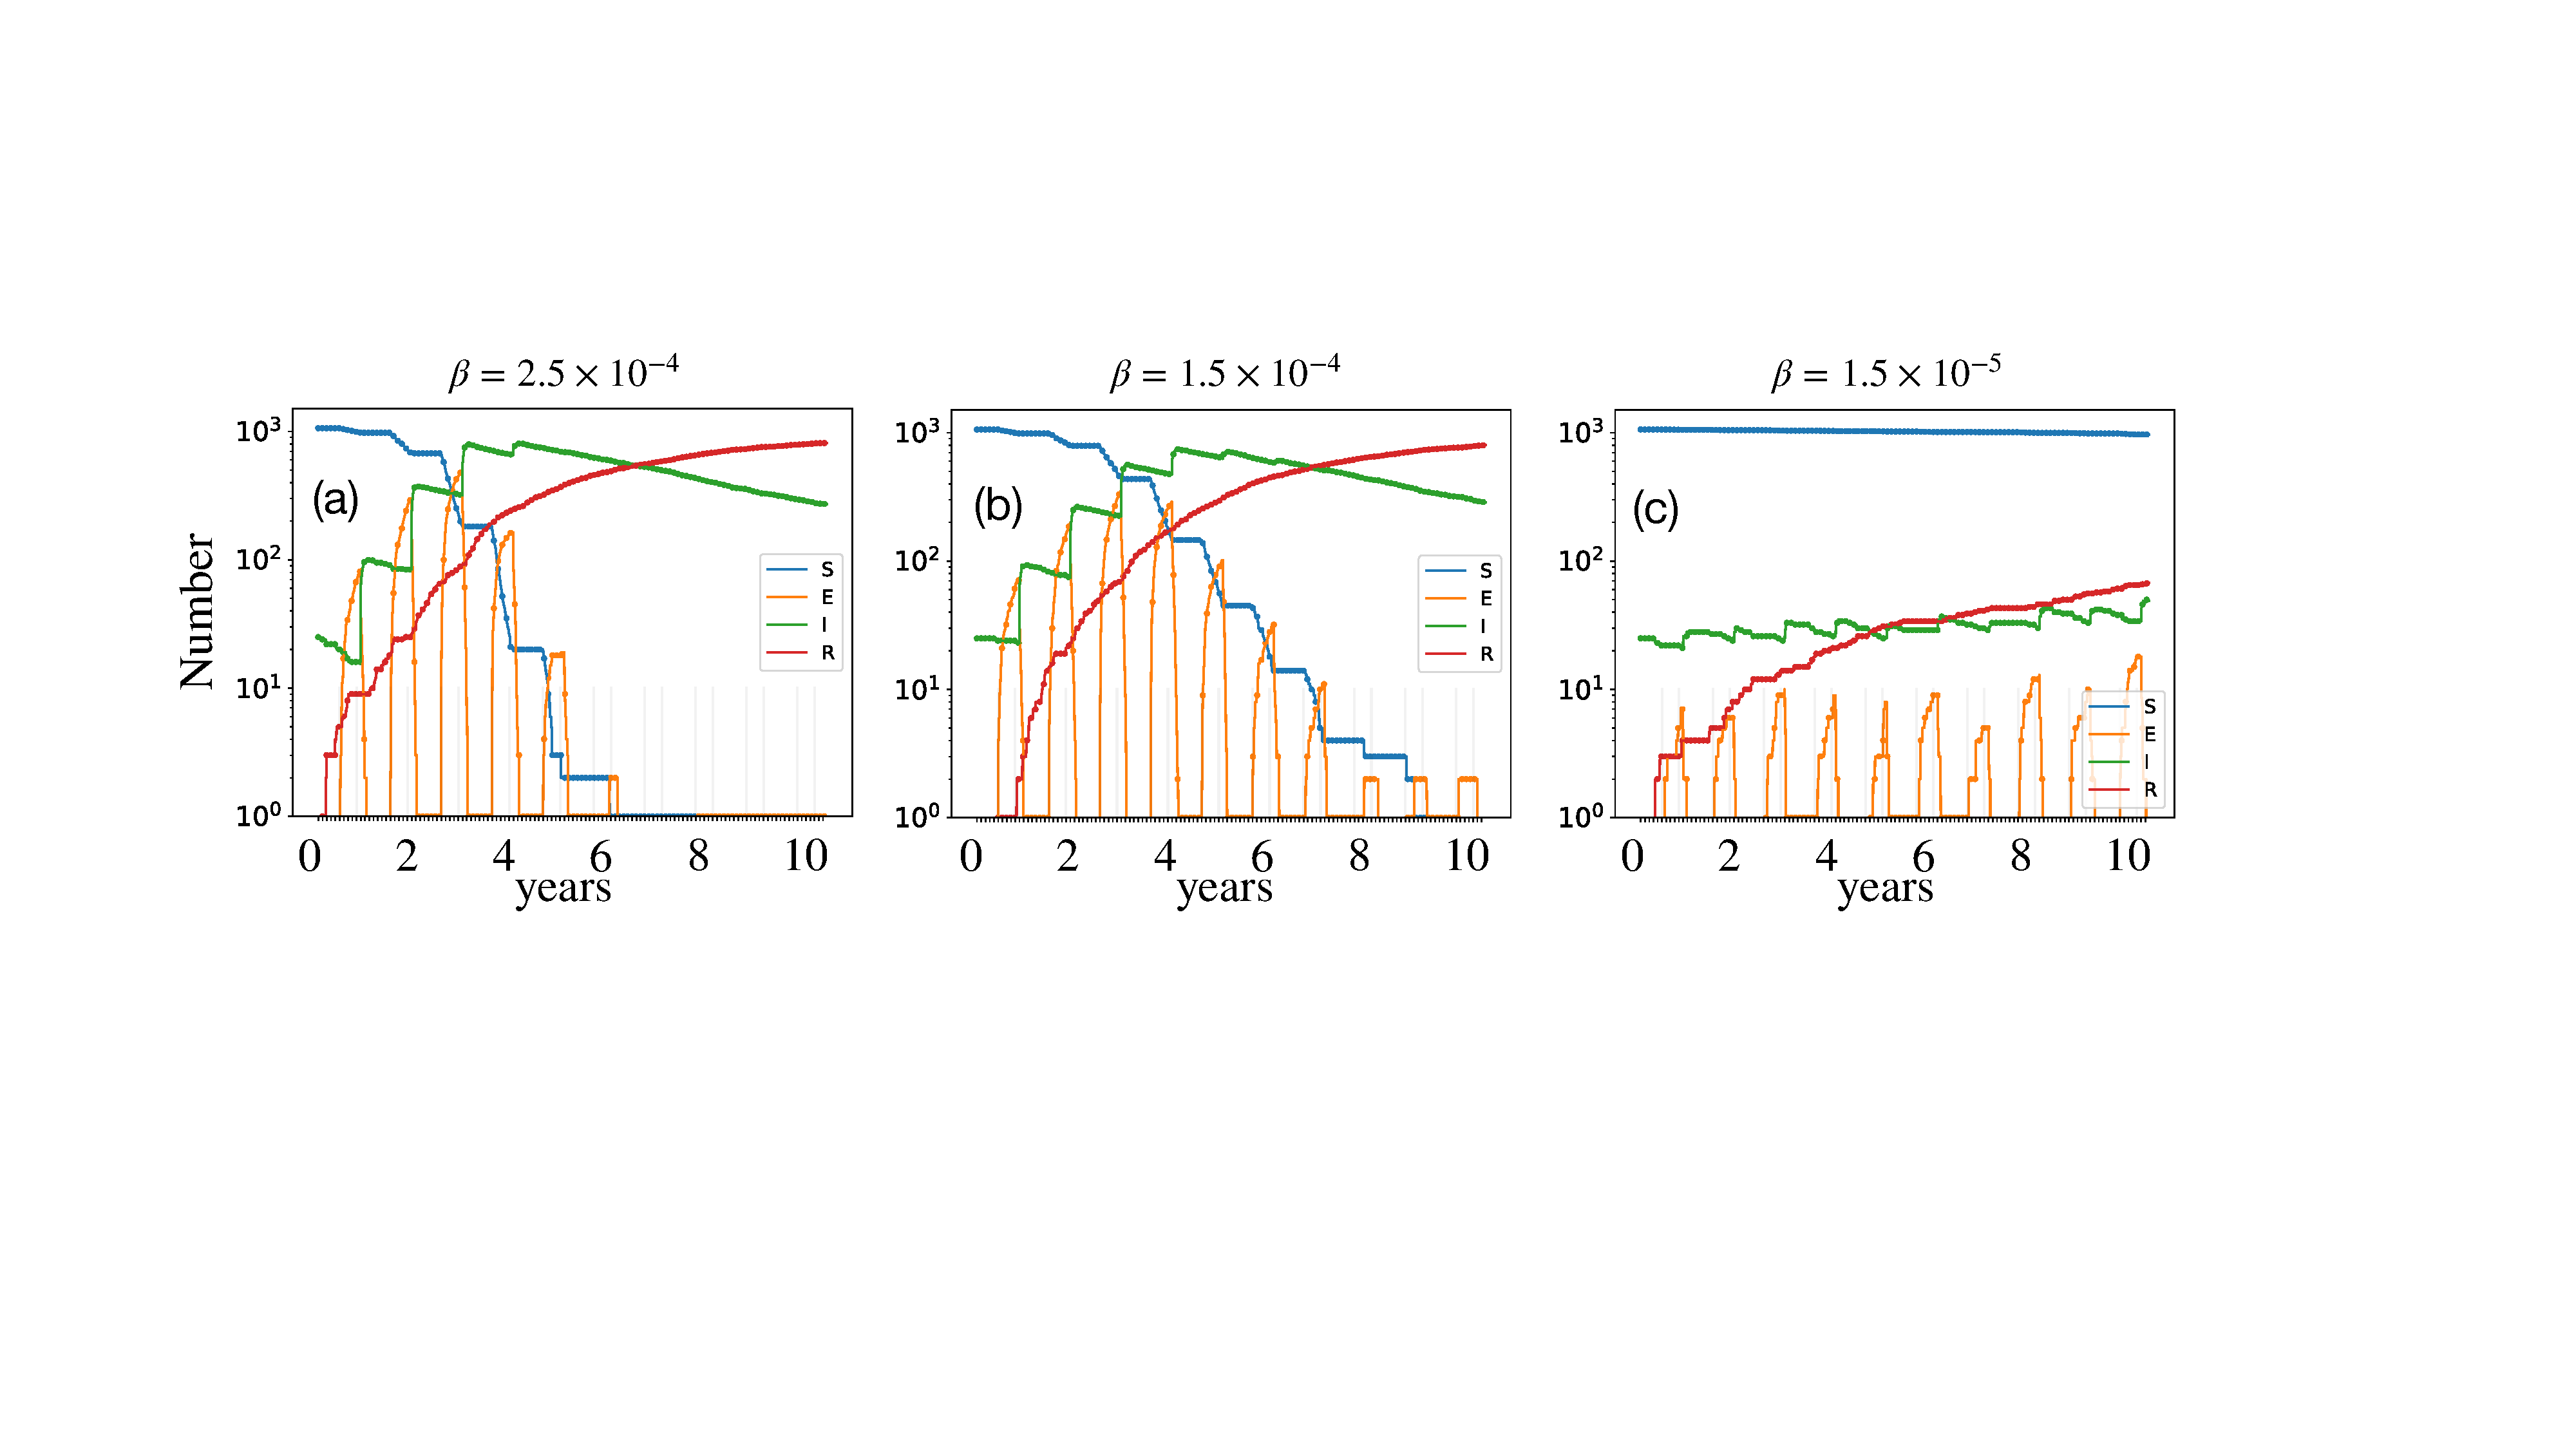
\includegraphics[scale=0.30]{appendix/figures/A-ch6-ga-seir.pdf}
    \caption{Ten year simulations of the Gaussian variant of seasonal the $SEIR$ model. (a-c) show three variations of infectivity $\beta$ over the average density of ash in Great Britain.}
    \label{fig-ga-SEIR-variant}
\end{figure}


\section{Defining an $R_0$}

\begin{figure}
    \centering
    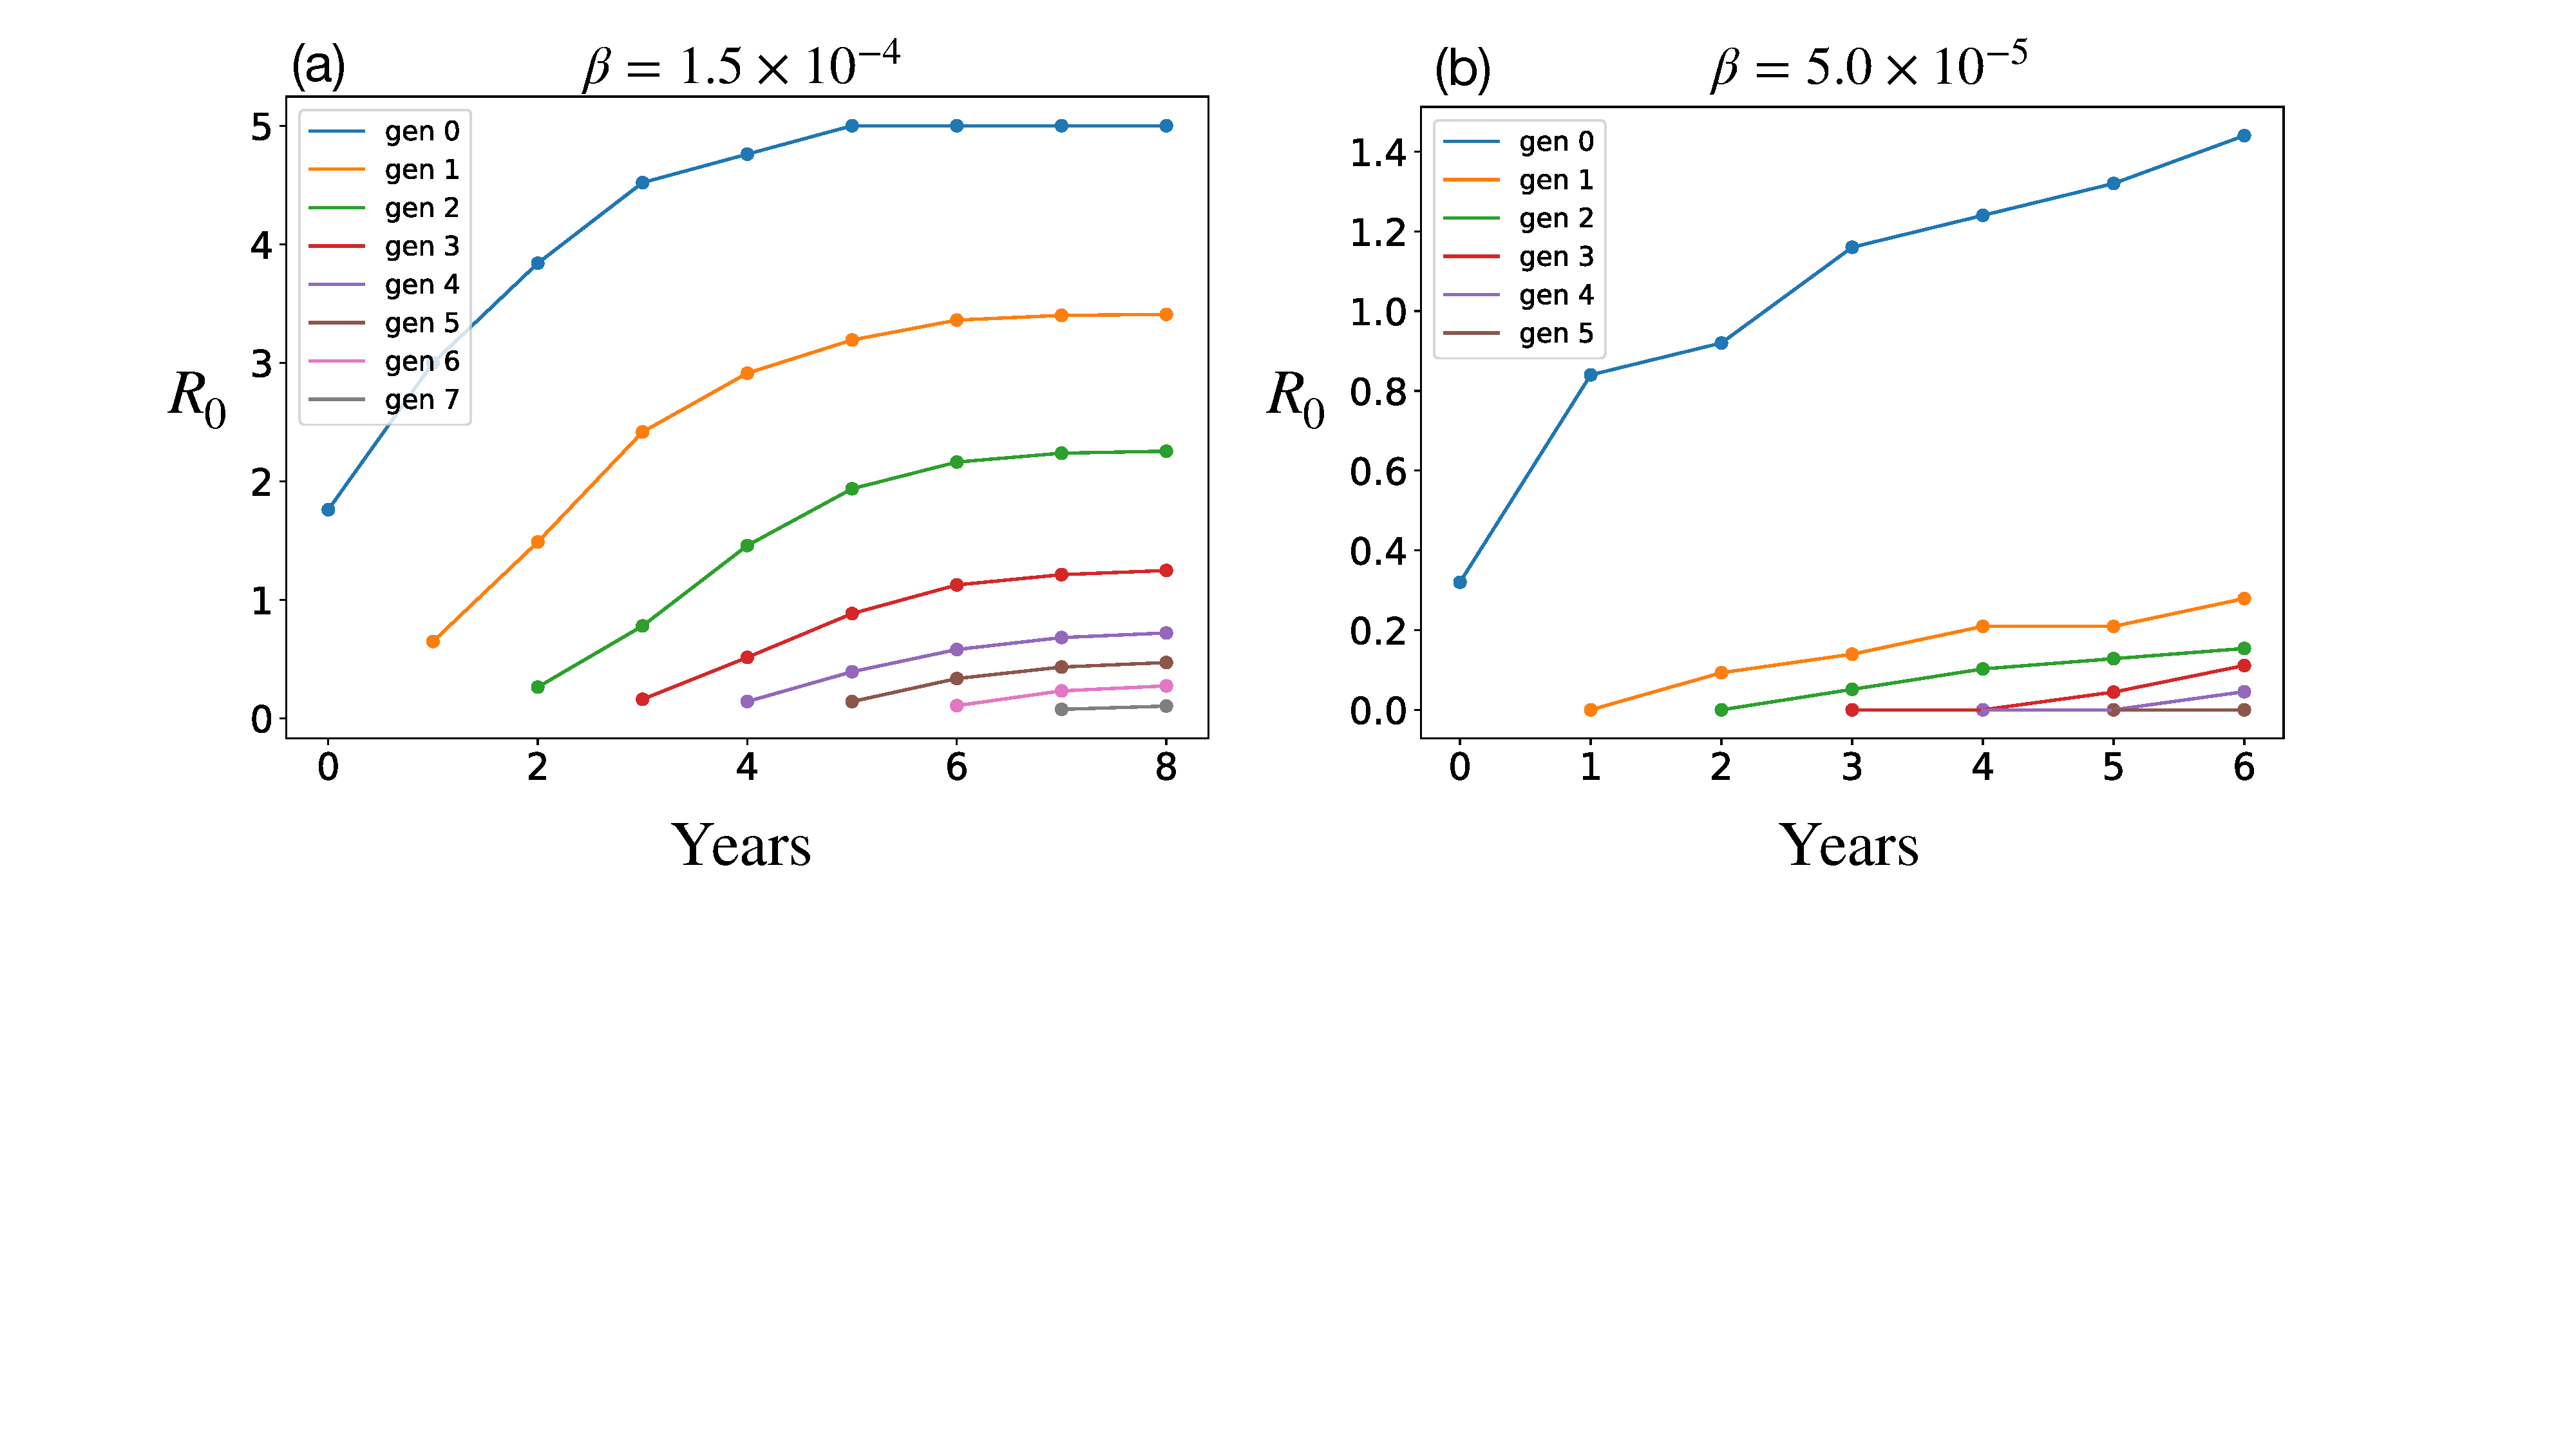
\includegraphics[scale=0.25]{appendix/figures/A-ch6-R0-saturation-with-beta.pdf}
    \caption{The average number of contact-traced secondary infections, $R_0$, saturating to the final value with time. (a) For a more invasive pathogen, it takes less time for $R_0$ to reach its final value (b) For a less invasive pathogen, it takes a longer time to saturate to the final value.}
    \label{fig:a-R0-saturate}
\end{figure}

\subsection{Seasonal $R_0$ measures}
For this $SEIR$ model of ADB, new secondary infections only occur during summertime sporulation which can be conveniently reflected by a seasonal average, $R_S$. The definition of $R_S$ for ADB can be stated as:
\begin{defn}
for years $(1,2.,,n)$ a series of ratios $(R_{1},R_2,...,R_{n})$ measure the mean number of secondary infections produced by an infectious ash over the sporulation season
\end{defn}
where 'mean' refers to the contact-traced number of infections produced by an individual as per Figure \ref{fig:contact-trace}.

In this model, the seasonal average $R_S$ is likely to underestimates the true value of $R_0$. This follows from the fact an infected ash tree has on average a life time of five years. It is widely accepted that policy makers should act quickly to a control an epidemic, and this observation once again highlights the challenge for policy makers because measuring $R_0$ over five years is likely to be too a time frame. However.


\subsection{Seasonal $SEIR$ with domain-size}
\label{a:seir-with-L}
\begin{figure}
    \centering
    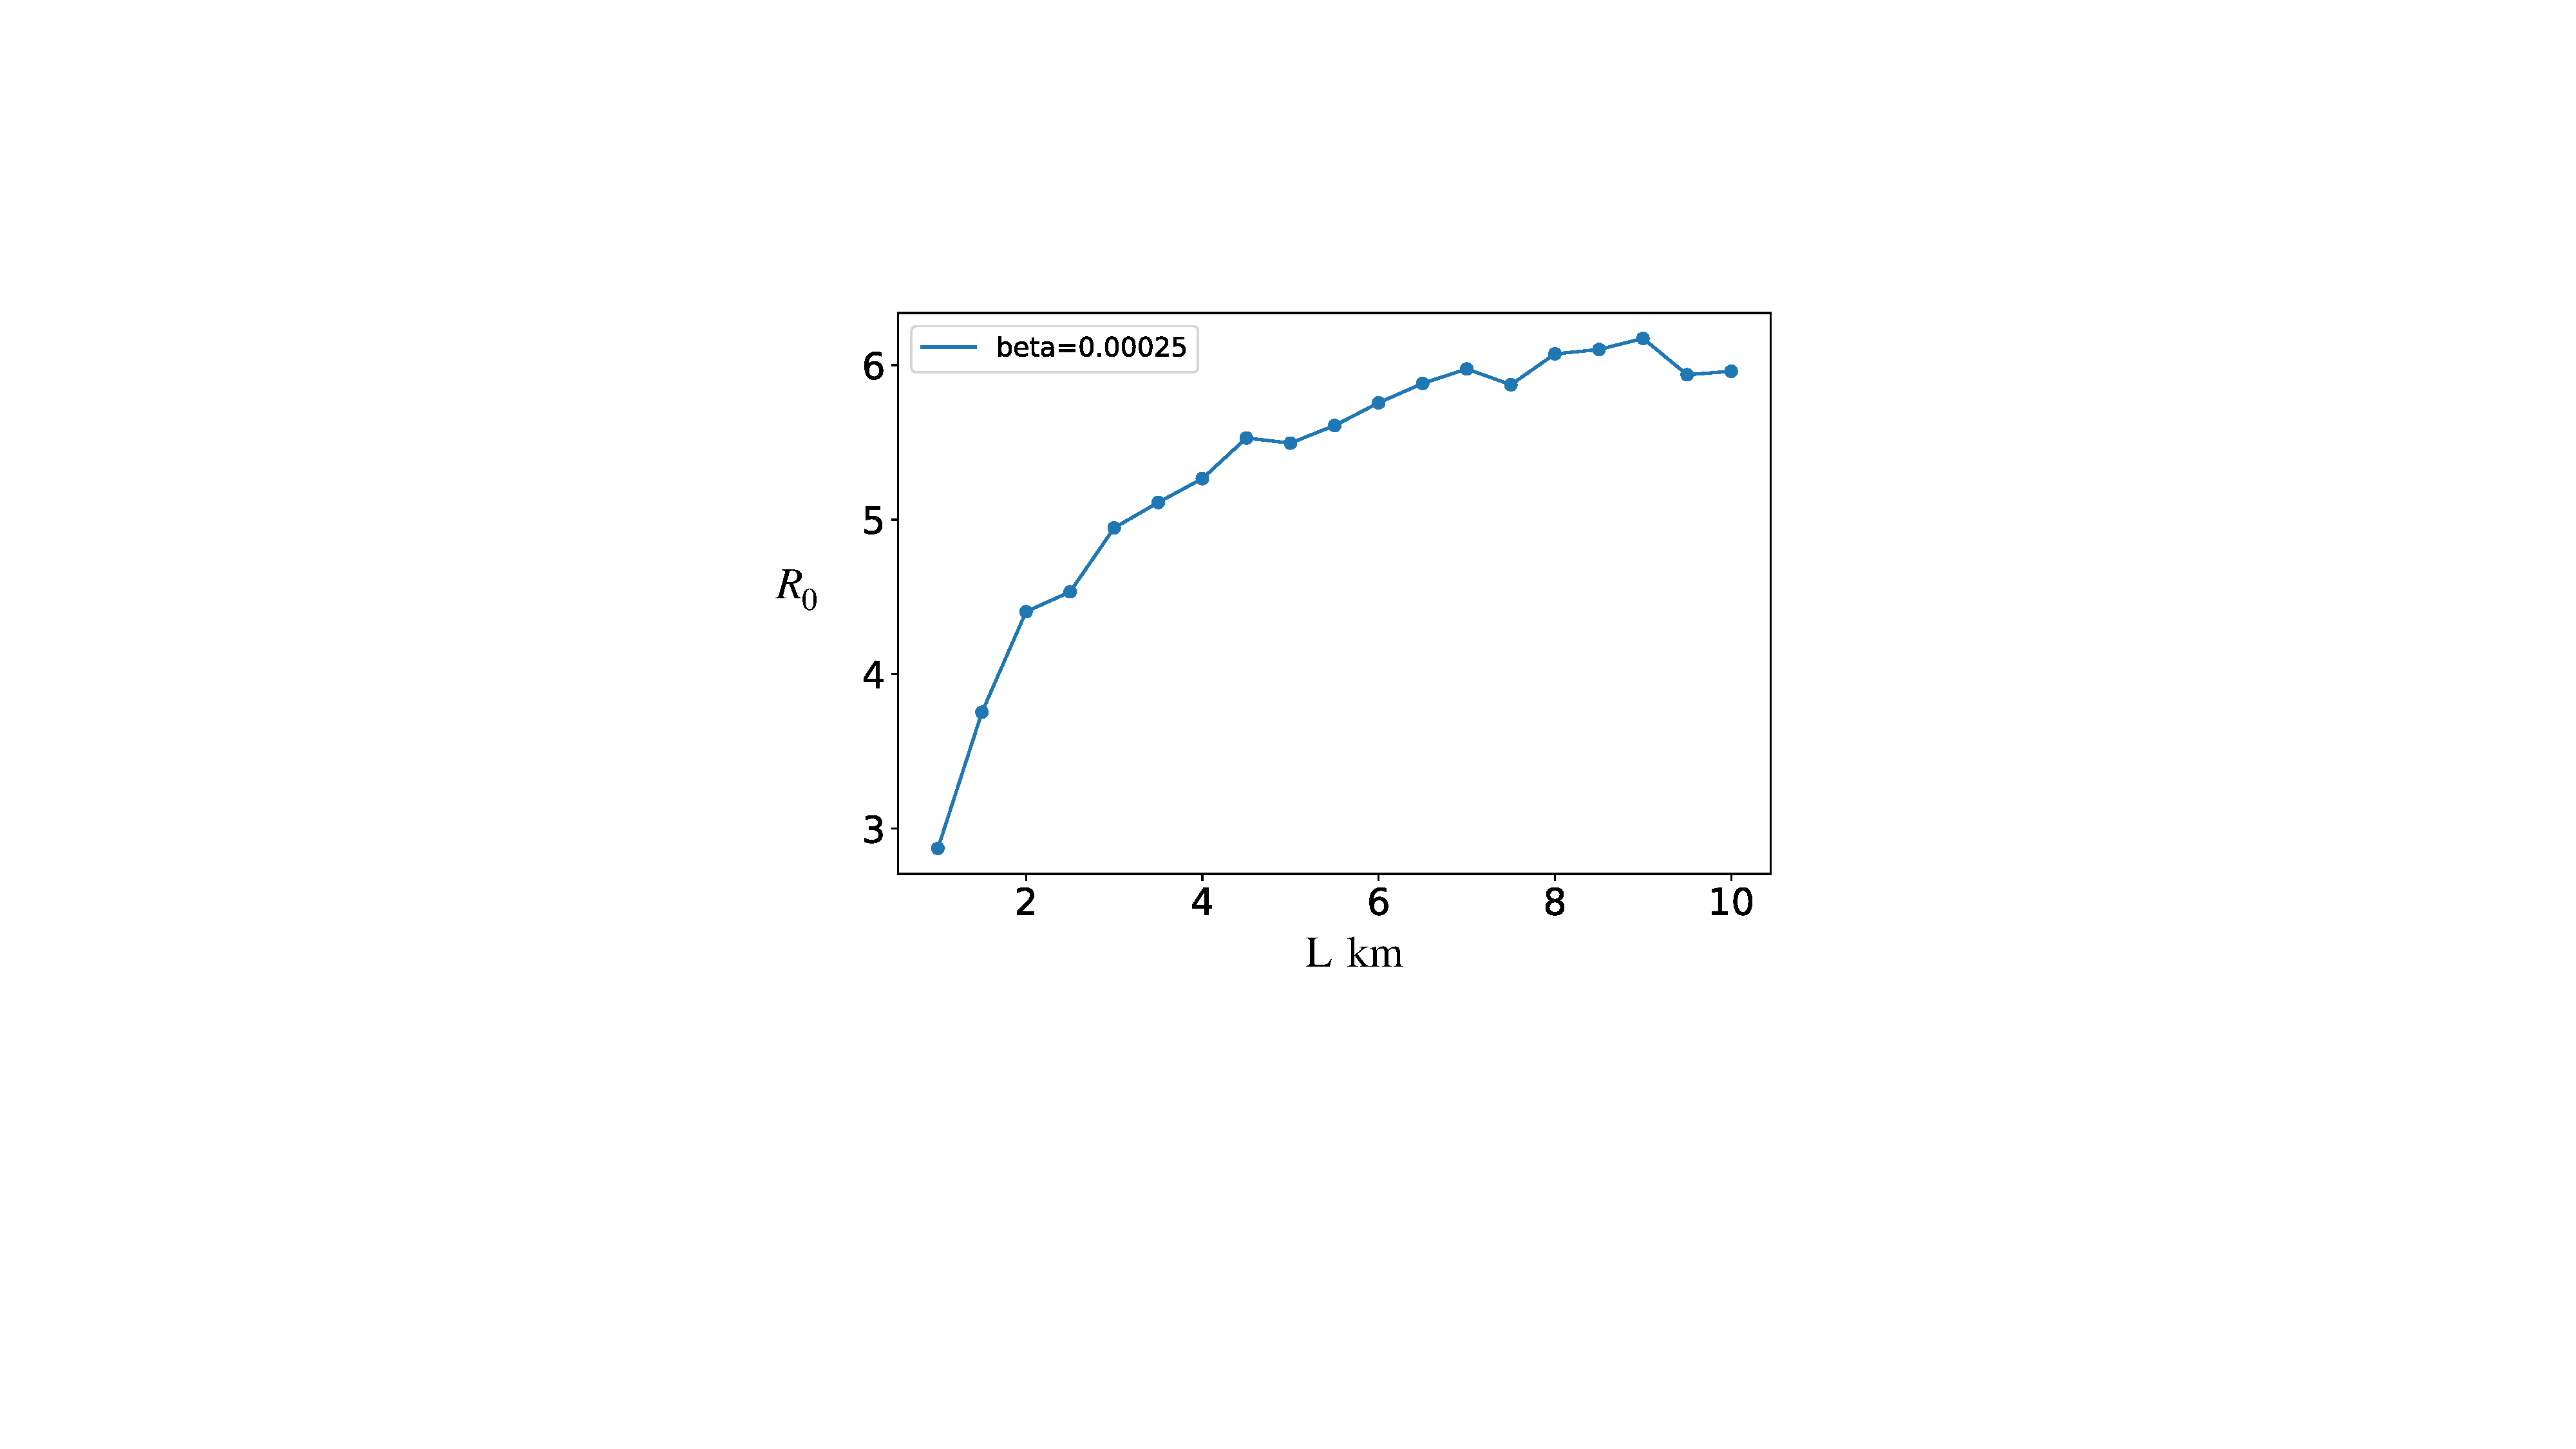
\includegraphics[scale=0.30]{appendix/figures/A-ch6-R0-vs0-L.pdf}
    \caption{The $10$ year mean $R_0$ value is shown against different domain sizes, $L$. The value of $R_0$ can be seen to start leveling off at around $5\mathrm{km} \times 5\mathrm{km}$. Beyond this point there is little difference in $R_0$, but considerable differences in the computational run-time.}
    \label{fig:a-R0-saturate-with-L}
\end{figure}
